\documentclass[../main/main.tex]{subfiles}

\newdate{date}{10}{06}{2020}

\begin{document}

\section{Lecture 22}
 \displaydate{date}. Compiled:  \today. Martina 

\subsubsection{Slide 376}

\begin{figure}[h!]
\centering
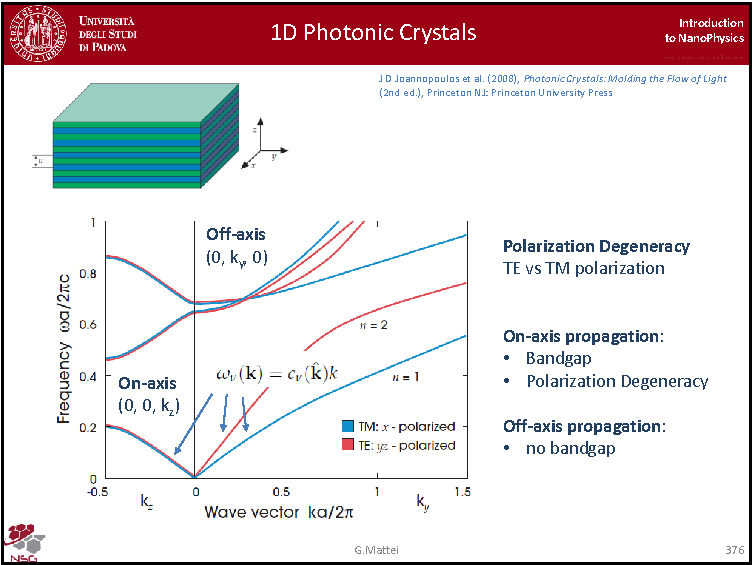
\includegraphics[page=1,width=0.9\textwidth]{../lessons/pdf_file/22_lesson.pdf}
\end{figure}


If we consider the effect of polarization on the propagation of light within 1D photonic crystals, we can calculate the dispersion law for a given situation.

For the on-axis propagation, that is propagation along the perpendicular direction whit respect to the interface of the multilayer, the k vector is aligned with the z direction and in this case polarization is irrelevant because we can rotate around that specific direction and this is invariant for rotation around the z axis, so we have degenerate bands for on-axis propagation, both for TE or TM polarization, that is the red or the blue curve.

Of course in this case we have this photonic bandgap as we have seen, but if we consider off-axis propagation in which we have non negligible component of the incident vector in a dimension which is not the z direction, in this case of course we have removal of the degeneracy and splitting of the degenerate bands, and in this case we have another interesting phenomenon, for which we could also have the disappear of the band gap for particular condition of incident beam. 

So in this case of course polarization has a major role in the propagation of light.

\newpage


\subsubsection{Slide 377}
 
 \begin{figure}[h!]
\centering
\includegraphics[page=2,width=0.9\textwidth]{../lessons/pdf_file/22_lesson.pdf}
\end{figure}

Another important fact in the variation of the periodicity is the presence of defects. 

You may remember that for the ordinary crystals the presence of defects can be considered as a perturbation of the Hamiltonian, so that instead of having the bandgap we have levels within the band gap, and in this case for instance if we have one of the layer which is no longer of the same thickness of the periodic layer, we can have an additional energy level in the gap, so that we can localize strongly the electromagnetic energy density in that specific defect, and in particular in this case we have a  very large component of the field along the z direction. 

So we can use defects to localize the electric field, because we have no longer perfectly extended modes in our crystal.

\newpage

\subsubsection{Slide 378}

\begin{figure}[h!]
\centering
\includegraphics[page=3,width=0.9\textwidth]{../lessons/pdf_file/22_lesson.pdf}
\end{figure}

We can look at the very same effect in the energy band diagram considering the density of states that can be calculated with the usual formula known from the solid state course. 

When you have the dispersion law you can calculate the gradient of the dispersion law which is nothing but the group velocity, take the modulus, take the inverse and integrate over an isosurface in which $\omega$ is constant and you sum over all the polarization in your system, and so you can calculate the density of allowed states.

Of course when you have the photonic bandgap you have no density of states, then you still have another allowed set of states and another photonic bandgap in which we do not have propagating states but only evanescent states, so that if you have defects you can obtain a defect state, that is for a specific value of $\omega$ you have propagation with a very strong localization, and you can of course obtain pass-band filters like in dielectric Fabry-Perot filter, perfect reflectors as we have seen and you can induce the defect to propagate according to your specific needs.

\newpage

\subsubsection{Slide 379}

\begin{figure}[h!]
\centering
\includegraphics[page=4,width=0.9\textwidth]{../lessons/pdf_file/22_lesson.pdf}
\end{figure}

Another important kind of defect is the surface, that is an interruption of the periodicity. 

In this case also for off-axiz propagation you can have no longer extended modes and you can have a strong localization of the field at the surface; with that trick you can use also dielectric photonic crystals to obtain an intense light confinement at the surface of your material. 

\newpage

\subsubsection{Slide 380}

\begin{figure}[h!]
\centering
\includegraphics[page=5,width=0.9\textwidth]{../lessons/pdf_file/22_lesson.pdf}
\end{figure}

What about increasing the dimensionality? That is, if we go from 2D crystals like self-assembled monolayer of dielectric spheres in 1D as we have seen, we have of course the optical semiconductors for light, like the 1D version, but in this case we have more rich set of dispersion laws.

\newpage

\subsubsection{Slide 381}

\begin{figure}[h!]
\centering
\includegraphics[page=6,width=0.9\textwidth]{../lessons/pdf_file/22_lesson.pdf}
\end{figure}

In this case for instance if we consider pillars in an ordered  arrays we can modulate the dielectric function in this case between the pillar and the air or the medium around, in the exact way in which we have those structures on the wings of butterfly, which mimics exactly the photonic crystal so that the color of the wings are not due to some pigments but due to the photonic crystal behaviour. 

We can obtain the very same effect by constructing an ordered arrays of pillars of silicon for instance on a silica matrix in order to have propagation of light exactly in prescribed patterns. 

\newpage

\subsubsection{Slide 382}

\begin{figure}[h!]
\centering
\includegraphics[page=7,width=0.9\textwidth]{../lessons/pdf_file/22_lesson.pdf}
\end{figure}

That is a very interesting topic because we can have specific direction according to the polarization.

In this case we can have for instance photonic bandgap for TM modes, in this case in which we have silicon rodes embedded in the air with a ratio of the radius versus the period which is around 0.80, and the transverse magnetic propagation is polarized in this direction while transverse electric is polarized in this direction.

So for TM modes we have as expected photonic bandgap, whereas for TE modes as we have seen we no longer have the band structure, so in this case polarization is a very important degree of freedom we can use to control light propagation.

\newpage

\subsubsection{Slide 383}

\begin{figure}[h!]
\centering
\includegraphics[page=8,width=0.9\textwidth]{../lessons/pdf_file/22_lesson.pdf}
\end{figure}

We can have also photonic crystal waveguides because if we have some defects in the stuck of our system or a line defect or a point defect, we can localize strongly the light. 

In this case we have photonic optical fiber in which the light is confined in those structures, this can be even more more complicated with a full hole core, photonic bandgap Fibers, in which the concept of cavity is of high relevance. 

\newpage

\subsubsection{Slide 385}

\begin{figure}[h!]
\centering
\includegraphics[page=9,width=0.9\textwidth]{../lessons/pdf_file/22_lesson.pdf}
\end{figure}

I will not enter in too many details but what I would like to show you is how to simply obtain photonic crystal waveguides by for instance promoting defects like the lack of a given set of a pillars in this particular case. 

If you remove the pillars in prescribed patterns you can guide light even to bend 90 degrees for instance, because in that case you have particular value of the wavelength or frequency for which we have guided modes within the bandgap and so you can obtain really very narrow confinement of light and propagation within prescribed even very crazy path.

\newpage

\subsubsection{Slide 386}

\begin{figure}[h!]
\centering
\includegraphics[page=10,width=0.9\textwidth]{../lessons/pdf_file/22_lesson.pdf}
\end{figure}

The situation is depicted here: we did a simulation of 2D photonic crystal waveguide in which the pillars are made of gallium arsenide with a very large refractive index of 13 (air has an index of dielectric function of 1, so a very large contrast). 

If we tune the lattice parameter of this square arrays of pillars, in this case 368 nm of periodicity, we can solve the Helmoltz equations with numerical technique and if we pump the system with an incoming wave here, we want to see if we are able to propagate the wave within this path and to move to this 90 degree bending. 

\newpage

\subsubsection{Slide 387}

\begin{figure}[h!]
\centering
\includegraphics[page=11,width=0.9\textwidth]{../lessons/pdf_file/22_lesson.pdf}
\end{figure}

This is the simulation in which we are evaluating the component of the electric field perpendicularly to the plane and in this case the red is positive ad the blue is negative.

So we can see the effect of propagation of light which goes back, which propagates exactly in the prescribed path provided that the wavelength matches the frequency of the localized state as the defect in the periodic array. 

Of course if the wavelength does not match the one of the defect, even small variations inverse the propagation as you can see here in which the light exponentially decays when tries to enter the waveguide. 

So this is a clear indication that the waveguide can be very frequency or wavelength selective in this particular case.

\newpage

\subsubsection{Slide 388}

\begin{figure}[h!]
\centering
\includegraphics[page=12,width=0.9\textwidth]{../lessons/pdf_file/22_lesson.pdf}
\end{figure}

We can also see the very same effect by looking at the Poynting vector modulus, that is the energy flow in the system, and if we plot the modulus of the Poynting vector we of course have this energy propagation. 

There is attenuation because the mode is quite leaky, so the wavelength is much larger than the path in which it is propagating, so the mode is leaky in the sense that some of the energy can disappear and can be dissipated, but of course if we need to bend light we can do it in a very effective way like in this technique, and you can see that in the case of resonant propagation there is no flow of energy in the system because we have an exponentially evanescent instead of a propagating wave with that specific device.

\newpage

\subsubsection{Slide 389}

\begin{figure}[h!]
\centering
\includegraphics[page=13,width=0.9\textwidth]{../lessons/pdf_file/22_lesson.pdf}
\end{figure}

The situation is even more complicated if we change the symmetry, not square but hexagonal symmetry like in this case. We can calculate the dispersion law according to the reciprocal direction in the Brillouin zone, that is in the $\Gamma K$ or $\Gamma M$ direction, but in this case we have seen a photonic bandgap.

\newpage

\subsubsection{Slide 390}

\begin{figure}[h!]
\centering
\includegraphics[page=14,width=0.9\textwidth]{../lessons/pdf_file/22_lesson.pdf}
\end{figure}

The 3D case is even more complicated. According to the structure we have or have not the photonic bandgap in the fcc, for instance if we have dielectric spheres in fcc structures we do not have a photonic bandgap whereas if we have the diamond lattice we have the photonic bandgap, so the symmetry plays an important role.

\newpage

\subsubsection{Slide 391}

\begin{figure}[h!]
\centering
\includegraphics[page=15,width=0.9\textwidth]{../lessons/pdf_file/22_lesson.pdf}
\end{figure}

Or if we have more exotic shapes, like the woodpile or the inverse opal, we can modulate the presence of the photonic bandgap and in a very narrow region we can obtain out of those systems very accurate filters, pass-band or perfect reflectors.

\newpage

\subsubsection{Slide 392-393}

\begin{figure}[h!]
\centering
\includegraphics[page=16,width=0.9\textwidth]{../lessons/pdf_file/22_lesson.pdf}
\end{figure}

\begin{figure}[h!]
\centering
\includegraphics[page=17,width=0.9\textwidth]{../lessons/pdf_file/22_lesson.pdf}
\end{figure}

\newpage

In perfect analogy as in the band structures for crystals of electrons, we obtained much larger scale photonic structures for photons by modulating not the coulomb potential but the dielectric function. In this case of the germanium we have the forbidden gap whereas in the case of copper we do not have a bandgap because we fill up to the Fermi level.

\clearpage

\end{document}